{\color{gray}

Código de identificação do voluntário: \rule{1in}{.2mm}

\textit{Os dados deste questionário são anônimos e somente serão utilizados para fins acadêmicos e de pesquisa, ficando proibido seu manuseio ou uso sem consentimento do coordenador da pesquisa.}
}

\begin{center}
\textbf{Parte 3 - Questionário sobre consciência situacional (SAGAT).}
\end{center}

\noindent
\textbf{TESTE} ( ) BASE \hfill ( ) ÁUDIO \hfill ( ) CINTO HÁPTICO \hfill ( ) BENGALA \hfill ( ) MISTO

\textbf{Primeira visita}

\hspace{0.5cm}

\begin{table}[!htb]
    \centering
    \begin{tabular}{m{0.5\linewidth} m{0.5\linewidth}}
        \large{Nível 1 – Percepção}  &\\
        & \\
        %---------------------------------
        1) Existe algum objeto próximo de você? & 2) Sinalize onde o objeto está: \\
        & \\
        \rule{\linewidth}{.2mm} & \begin{center}\multirow{5}{*}{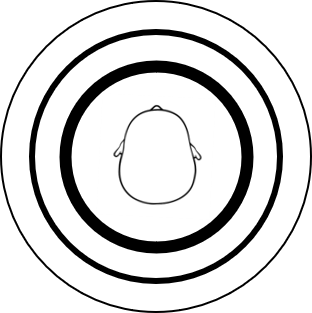
\includegraphics[width = 0.45\linewidth]{ApendC_(Questionarios)/diagrama_sagat.png}} \end{center}\\
        \rule{\linewidth}{.2mm} & \\
        & \\
        \rule{\linewidth}{.2mm} & \\
        & \\
        \rule{\linewidth}{.2mm} & \\
        & \\
\end{tabular}
\end{table}
\begin{table}[!htb]
    \begin{tabular}{m{0.5\linewidth} m{0.5\linewidth}}
         %---------------------------------
         3)	Existe alguém perto de você? & 4) Sinalize onde a pessoa está: \\
        & \\
        \rule{\linewidth}{.2mm} & \begin{center}\multirow{5}{*}{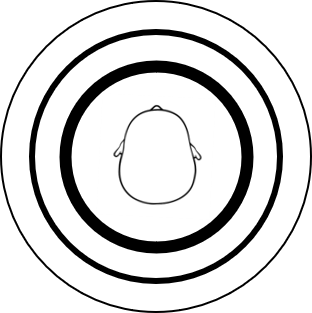
\includegraphics[width = 0.45\linewidth]{ApendC_(Questionarios)/diagrama_sagat.png}} \end{center}\\
        \rule{\linewidth}{.2mm} & \\
        & \\
        \rule{\linewidth}{.2mm} & \\
        & \\
        \rule{\linewidth}{.2mm} & \\
        & \\
\end{tabular}
\end{table}
\begin{table}[!htb]
    \begin{tabular}{m{0.5\linewidth} m{0.5\linewidth}}
        %---------------------------------
         5)	Você percebeu alguma fonte de som característica do lugar onde você se encontra? & 6)	Sinalize de onde vem o som: \\
        & \\
        \rule{\linewidth}{.2mm} & \begin{center}\multirow{5}{*}{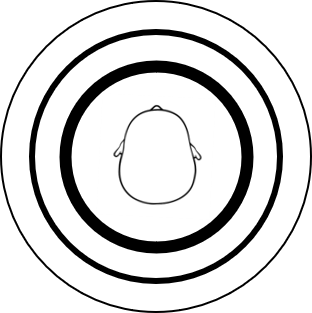
\includegraphics[width = 0.45\linewidth]{ApendC_(Questionarios)/diagrama_sagat.png}} \end{center}\\
        \rule{\linewidth}{.2mm} & \\
        & \\
        \rule{\linewidth}{.2mm} & \\
        & \\
        \rule{\linewidth}{.2mm} & \\
        & \\
        %---------------------------------
    \end{tabular}
\end{table}
\begin{table}[!htb]
    \begin{tabular}{m{0.5\linewidth} m{0.5\linewidth}}
        %---------------------------------
        \large{Nível 2 – Compreensão}  &\\
        & \\
        & \\
        %---------------------------------
        7)	Sinalize em que direção está a recepcionista: & 8)	Sinalize em que direção está a saída: \\
        & \\
        \begin{center}\multirow{5}{*}{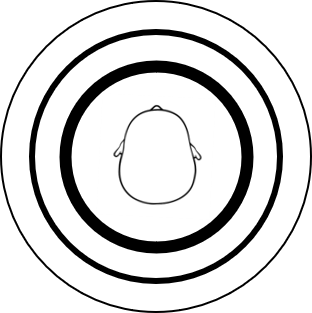
\includegraphics[width = 0.45\linewidth]{ApendC_(Questionarios)/diagrama_sagat.png}} \end{center} & \begin{center}\multirow{5}{*}{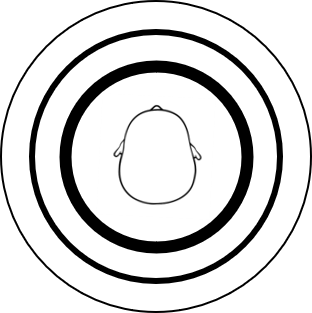
\includegraphics[width = 0.45\linewidth]{ApendC_(Questionarios)/diagrama_sagat.png}} \end{center}\\
        & \\
        & \\
        & \\
        & \\
        & \\
        %---------------------------------
    \end{tabular}
\end{table}
\begin{table}[!htb]
    \begin{tabular}{m{0.5\linewidth} m{0.5\linewidth}}
        %---------------------------------
        \large{Nível 3 – Projeção}  &\\
        & \\
        & \\
        %---------------------------------
        9)	O que você espera encontrar no caminho ao retornar à mesa de recepção? & 10)	Qual será a sua trajetória para sair? Descreva seus próximos movimentos. \\
        & \\
        \rule{\linewidth}{.2mm} & \rule{\linewidth}{.2mm}\\
        & \\
        \rule{\linewidth}{.2mm} & \rule{\linewidth}{.2mm}\\
        & \\
        \rule{\linewidth}{.2mm} & \rule{\linewidth}{.2mm}\\
        & \\
        \rule{\linewidth}{.2mm} & \\
        & \\
\end{tabular}
\end{table}
\begin{table}[!htb]
    \begin{tabular}{m{0.5\linewidth} m{0.5\linewidth}}
        %---------------------------------
        11)	Qual a distância você imagina que existe entre você e a mesa da recepção? & 12)	Qual a distância você imagina que existe entre você e a saída? \\
        & \\
        \rule{\linewidth}{.2mm} & \rule{\linewidth}{.2mm}\\
        & \\
        \rule{\linewidth}{.2mm} & \rule{\linewidth}{.2mm}\\
        & \\
        \rule{\linewidth}{.2mm} & \rule{\linewidth}{.2mm}\\
        & \\
        \rule{\linewidth}{.2mm} & \\
        & \\
        %---------------------------------
    \end{tabular}
\end{table}



\FloatBarrier

\textbf{Retorno}

\hspace{0.5cm}

\begin{table}[!htb]
    \centering
    \begin{tabular}{m{0.5\linewidth} m{0.5\linewidth}}
        \large{Nível 1 – Percepção}  &\\
        & \\
        %---------------------------------
        1) Existe algum objeto próximo de você? & 2) Sinalize onde o objeto está: \\
        & \\
        \rule{\linewidth}{.2mm} & \begin{center}\multirow{5}{*}{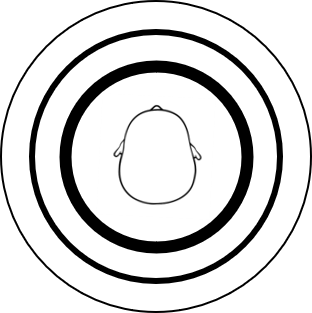
\includegraphics[width = 0.45\linewidth]{ApendC_(Questionarios)/diagrama_sagat.png}} \end{center}\\
        \rule{\linewidth}{.2mm} & \\
        & \\
        \rule{\linewidth}{.2mm} & \\
        & \\
        \rule{\linewidth}{.2mm} & \\
        & \\
\end{tabular}
\end{table}
\begin{table}[!htb]
    \begin{tabular}{m{0.5\linewidth} m{0.5\linewidth}}
         %---------------------------------
         3)	Existe alguém perto de você? & 4) Sinalize onde a pessoa está: \\
        & \\
        \rule{\linewidth}{.2mm} & \begin{center}\multirow{5}{*}{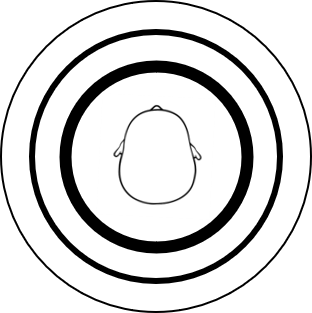
\includegraphics[width = 0.45\linewidth]{ApendC_(Questionarios)/diagrama_sagat.png}} \end{center}\\
        \rule{\linewidth}{.2mm} & \\
        & \\
        \rule{\linewidth}{.2mm} & \\
        & \\
        \rule{\linewidth}{.2mm} & \\
        & \\
\end{tabular}
\end{table}
\begin{table}[!htb]
    \begin{tabular}{m{0.5\linewidth} m{0.5\linewidth}}
        %---------------------------------
         5)	Você percebeu alguma fonte de som característica do lugar onde você se encontra? & 6)	Sinalize de onde vem o som: \\
        & \\
        \rule{\linewidth}{.2mm} & \begin{center}\multirow{5}{*}{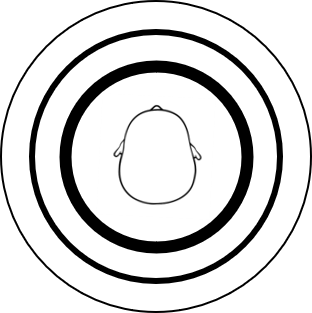
\includegraphics[width = 0.45\linewidth]{ApendC_(Questionarios)/diagrama_sagat.png}} \end{center}\\
        \rule{\linewidth}{.2mm} & \\
        & \\
        \rule{\linewidth}{.2mm} & \\
        & \\
        \rule{\linewidth}{.2mm} & \\
        & \\
        %---------------------------------
    \end{tabular}
\end{table}
\begin{table}[!htb]
    \begin{tabular}{m{0.5\linewidth} m{0.5\linewidth}}
        %---------------------------------
        \large{Nível 2 – Compreensão}  &\\
        & \\
        & \\
        %---------------------------------
        7)	Sinalize em que direção está a recepcionista: & 8)	Sinalize em que direção está a saída: \\
        & \\
        \begin{center}\multirow{5}{*}{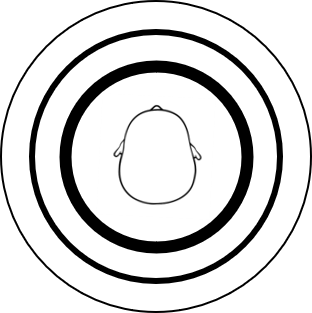
\includegraphics[width = 0.45\linewidth]{ApendC_(Questionarios)/diagrama_sagat.png}} \end{center} & \begin{center}\multirow{5}{*}{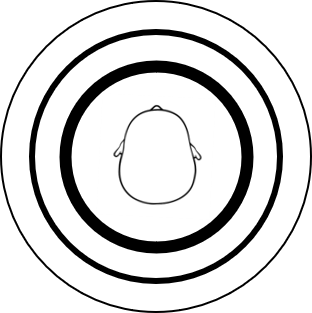
\includegraphics[width = 0.45\linewidth]{ApendC_(Questionarios)/diagrama_sagat.png}} \end{center}\\
        & \\
        & \\
        & \\
        & \\
        & \\
        %---------------------------------
    \end{tabular}
\end{table}
\begin{table}[!htb]
    \begin{tabular}{m{0.5\linewidth} m{0.5\linewidth}}
        %---------------------------------
        \large{Nível 3 – Projeção}  &\\
        & \\
        & \\
        %---------------------------------
        9)	O que você espera encontrar no caminho ao retornar à mesa de recepção? & 10)	Qual será a sua trajetória para sair? Descreva seus próximos movimentos. \\
        & \\
        \rule{\linewidth}{.2mm} & \rule{\linewidth}{.2mm}\\
        & \\
        \rule{\linewidth}{.2mm} & \rule{\linewidth}{.2mm}\\
        & \\
        \rule{\linewidth}{.2mm} & \rule{\linewidth}{.2mm}\\
        & \\
        \rule{\linewidth}{.2mm} & \\
        & \\
\end{tabular}
\end{table}
\begin{table}[!htb]
    \begin{tabular}{m{0.5\linewidth} m{0.5\linewidth}}
        %---------------------------------
        11)	Qual a distância você imagina que existe entre você e a mesa da recepção? & 12)	Qual a distância você imagina que existe entre você e a saída? \\
        & \\
        \rule{\linewidth}{.2mm} & \rule{\linewidth}{.2mm}\\
        & \\
        \rule{\linewidth}{.2mm} & \rule{\linewidth}{.2mm}\\
        & \\
        \rule{\linewidth}{.2mm} & \rule{\linewidth}{.2mm}\\
        & \\
        \rule{\linewidth}{.2mm} & \\
        & \\
        %---------------------------------
    \end{tabular}
\end{table}



\FloatBarrier
\pagebreak

%{\large Nível 1 – Percepção}
%
%1) Existe algum objeto próximo de você?
%
%\noindent
%\rule{6in}{.2mm} \\
%\rule{6in}{.2mm} \\
%\rule{6in}{.2mm}
%
%2) Sinalize onde o objeto está:
%
%%width=\textwidth
\begin{figure}[!h]
    \centering
    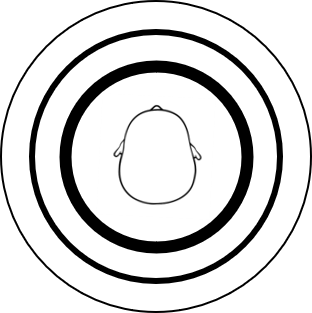
\includegraphics[scale=0.9]{ApendC_(Questionarios)/diagrama_sagat.png}
\end{figure}

\FloatBarrier
% 
%3) Existe alguém perto de você?
%
%\noindent
%\rule{6in}{.2mm} \\
%\rule{6in}{.2mm} \\
%\rule{6in}{.2mm}
%
%4) A pessoa está parada ou em movimento?
%
%\noindent
%\rule{6in}{.2mm} \\
%\rule{6in}{.2mm} \\
%\rule{6in}{.2mm}
%
%5) Sinalize onde a pessoa está:
%
%%width=\textwidth
\begin{figure}[!h]
    \centering
    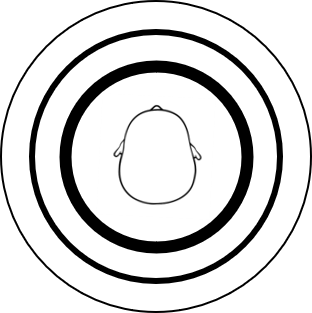
\includegraphics[scale=0.9]{ApendC_(Questionarios)/diagrama_sagat.png}
\end{figure}

\FloatBarrier 
%
%6) Você percebeu alguma fonte de som característica do lugar onde você se encontra?
%
%\noindent
%\rule{6in}{.2mm} \\
%\rule{6in}{.2mm} \\
%\rule{6in}{.2mm}
%
%7) Sinalize de onde vem o som:
% 
%\noindent
%\rule{6in}{.2mm} \\
%\rule{6in}{.2mm} \\
%\rule{6in}{.2mm}
% 
%{\large Nível 2 – Compressão}
%
%1) Sinalize em que direção está a recepcionista:
% 
%%width=\textwidth
\begin{figure}[!h]
    \centering
    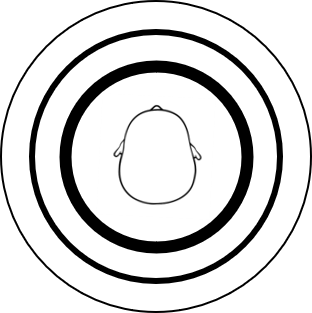
\includegraphics[scale=0.9]{ApendC_(Questionarios)/diagrama_sagat.png}
\end{figure}

\FloatBarrier 
% 
%2) Sinalize em que direção está a saída:
% 
%%width=\textwidth
\begin{figure}[!h]
    \centering
    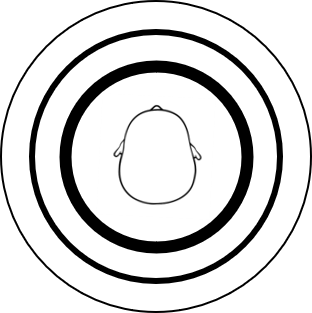
\includegraphics[scale=0.9]{ApendC_(Questionarios)/diagrama_sagat.png}
\end{figure}

\FloatBarrier 
%
%3) Sinalize em que direção está a sala de espera:
%
%%width=\textwidth
\begin{figure}[!h]
    \centering
    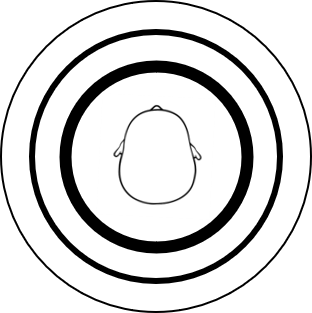
\includegraphics[scale=0.9]{ApendC_(Questionarios)/diagrama_sagat.png}
\end{figure}

\FloatBarrier  
%
%{\large Nível 3 – Projeção}
%
%1) O que você espera encontrar no caminho ao retornar à mesa de recepção?
%
%\noindent
%\rule{6in}{.2mm} \\
%\rule{6in}{.2mm} \\
%\rule{6in}{.2mm}
%
%2) Qual será a sua trajetória para sair? Descreva seus próximos movimentos.
%
%\noindent
%\rule{6in}{.2mm} \\
%\rule{6in}{.2mm} \\
%\rule{6in}{.2mm}
%
%3) Qual a distância você imagina que existe entre você e a mesa da recepção?
%
%\noindent
%\rule{6in}{.2mm} \\
%\rule{6in}{.2mm} \\
%\rule{6in}{.2mm}
%
%4) Qual a distância você imagina que existe entre você e a saída?
%
%\noindent
%\rule{6in}{.2mm} \\
%\rule{6in}{.2mm} \\
%\rule{6in}{.2mm}